\documentclass[11 pt, a4paper]{article}

% Fonts and math (Elsevier-like Times style)
\usepackage{newtxtext,newtxmath}
\usepackage{graphicx} % Required for inserting images
\usepackage{array} % For extra column formatting
\usepackage{amsmath} % for equation environment
\usepackage{float}
\usepackage{listings}
\usepackage{xcolor}
\usepackage{parskip} % For gaps between para
\usepackage{setspace}
\PassOptionsToPackage{hyphens}{url}\usepackage{hyperref}
\usepackage{makecell}
\usepackage[labelfont=bf]{caption}

% --- Abstract styling (elsarticle look)
\usepackage{abstract}
\renewcommand{\abstractnamefont}{\normalfont\bfseries}
\renewcommand{\abstracttextfont}{\normalfont}
\renewenvironment{abstract}{%
  \par\noindent\rule{\linewidth}{0.4pt}\par
  \begin{center}\bfseries Abstract\end{center}%
}{%
  \par\rule{\linewidth}{0.4pt}\par
}

% --- Section styling (similar to elsarticle)
\usepackage{titlesec}
\titleformat{\section}{\normalfont\large\bfseries}{\thesection.}{0.5em}{}
\titleformat{\subsection}{\normalfont\normalsize\bfseries}{\thesubsection.}{0.5em}{}

\title{\bfseries Orbits in the Solar System}
\author{Lian Fernandes}
\date{\today}

% --- Title info ---
\title{%

\includegraphics[width=0.9\linewidth]{UCD_Logo.png}\\ % Logo
{\large PHYC30170 Physics Astronomy and Space Lab I}\\ % Course info
{\bfseries Comparing Computational Methods for the Orbits in the Solar System} % Report title
}
\author{Lian Fernandes \\ \small Student No.: 22206311}
\date{09 September 2025}

% Python code export
\lstset{
    language=Python,
    basicstyle=\ttfamily\footnotesize,
    keywordstyle=\color{blue},
    commentstyle=\color{gray},
    stringstyle=\color{red},
    showstringspaces=false,
    frame=single,
    breaklines=true,
    numbers=left,
    numberstyle=\tiny\color{gray}
}

\begin{document}

\maketitle

\begin{abstract}

The aim of this experiment is to compare different computational methods for a more accurate orbit movement.

\end{abstract}

\section{Introduction}
Classical mechanics has been an intriguing study in the field of physics with it heavily being involved in the movement
of the planets in the solar system. Some of the most fundamental concepts involved in classical mechanics are Newton's Law
of Gravitation, centripetal forces of orbits and Kepler's Laws (in particular, Kepler's Third Law). The complexity of the orbits
of the solar system makes it hard and tedious to solve differential equations numerically. However, relating these equations with
numerical methods allow accuracy in answers and repeated coding.

As science has evolved with technology, solving complex differential equations has been much easier with the help of programming languages 
such as Python, C++, Java and more. In this paper, Python has been used throughout with libraries such as numpy, scipy and matplotlib
aiding with analysis and visualisation. With the help of these services, it is easier to model the orbits of the solar system and predict
the behaviour and trajectory of the celestial objects when in such system. This experiment simulated the orbital motion of celestial bodies 
around the Sun using numerical methods (Euler-Cromer and 2nd order Runge-Kutta) and explored the accuracy of these methods under different conditions.

\subsection{Orbital Mechanics}
Orbital mechanics are modeled using Newton's gravitational law and laws of motion alongside Kepler's law of motion. [1] Newton's gravitational 
law states that every object in the Universe is attracted to another object with a mass. [2] The equation that relates this is

\[
F = G \frac{m_1m_2}{r^2}
\tag{Eq. 1a}
\]

where \textbf{F} is the gravitational force between the two objects, $m_1m_2$ is the masses of the two objects, \textit{r} is the distance 
between the objects' centers and \textit{G} is the gravitational constant ($6.647 \times 10^{-11}$ m$^2$/kg$^2$). In relation to our Solar 
System, the Sun is in the middle of the system with celestial bodies (planets, comets, etc.) revolving around it. Due to this, the equation 
becomes

\[
\mathbf{F} = -\frac{GmM}{|r|^3}\mathbf{r}
\tag{Eq. 1b}
\]

where \textit{M} is the mass of the Sun.

Using Newton's second law of motion, $F=ma$, the equation for the acceleration of a celestial body, \textbf{a}(t), can be obtained assuming 
the Sun is stationary at the centre.

\[
\mathbf{a}(t) = -\frac{GM}{|\mathbf{r}(t)|^3}\mathbf{r}(t)
\tag{Eq. 2}
\]

where $r = \sqrt{x^2 +y^2}$.
The negative sign indicates that the force is in inwards and directed to the Sun. Newton's third law which states that every action has an 
equal and opposite reaction, can also be seen here. The gravitational force obtained supplies the centripetal force which keeps the body in 
orbit. [3] This provides the equation
\[
\frac{GMm}{R^2} = \frac{mv^2}{R}
\tag{Eq. 3}
\]
where \textbf{R} is the radius of the orbit.

The orbit of most celestial bodies are elliptical. However, some bodies do have circular orbits. All objects that have a circular orbit have a
circular velocity, \textit{v}, of
\[
v = \sqrt{\frac{GM}{R}}
\tag{Eq. 4}
\]
to keep the body in a stable orbit.

Kepler's laws are just as fundamental to orbital mechanics as Newton's laws of motion. [4] They are stated as follows:
\begin{itemize}
    \item \textit{Kepler's First Law:} The planet's orbit around the Sun is an elliptical orbit. Due the Sun's gravitational pull, the orbit of the bodies ends up as an ellipse.
    \item \textit{Kepler's Second Law:} Often called the law of equal areas. The line that joins the body and the Sun sweeps out equal areas in equal time intervals.
    \item \textit{Kepler's Third Law:} The squares of the orbital periods of the planets are proportional to the cubes of their semi-major axes.
\end{itemize}

In this experiment, Kepler's third law is prominent and can be used to calculate the planet's trajectories. The equation that follows this is
\[
\left(\frac{P_1}{P_2}\right)^2 = \left(\frac{a_1}{a_2}\right)^3
\tag{Eq. 5}
\]
where $P$ is the period of the orbit in years and $a$ is the semimajor axis.

Along with the laws of motion, conversation of energy is key in showing that the n-body system maintains its orbits and its
energy. Kinetic energy (KE) is the energy that the celestial body holds due to its motion. The equation for the KE is
\[
KE = \frac{1}{2}mv^2
\tag{Eq. 6}
\]
where $m$ is the mass of the body and $v$ is the total velocity in the x and y coordinate. The potential energy (PE) of the body is caused due
to the planet's location in the system. [5] The equation is as Eq. 1b.

Adding Eq. 1b and Eq. 6 equates to the total mechanical energy of the system and shows that mass is conserved.

For a binary (two stars) system with masses of $M_1$ and $M_2$, the total sum of the acceleration becomes
\[
\mathbf{a}(t) = -G\left(\frac{M_1}{(|r - r_1|)^3}(r - r_1) + \frac{M_2}{(|r - r_2|)^3}(r - r_2)\right)
\tag{Eq. 7}
\]

Energy is still conserved in such system.

\subsection{Euler-Cromer Method}
The Euler-Cromer method is an modified version of the Euler method that solves ordinary dfferential equations (ODEs) for various oscillatory 
systems. For an orbital system, this computes the vector position (r) and the velocity, $v$, of the body as

\begin{align}
\mathbf{v}(t+\Delta t) &= \mathbf{v}(t) + \Delta t\mathbf{a}(t) \tag{Eq. 8a}\\
\mathbf{r}(t+\Delta t) &= \mathbf{r}(t) + \Delta t\mathbf{v}(t+\Delta t) \tag{8b}
\end{align}

where $\Delta t$ is the time step, $\mathbf{v}$ is the velocity vector, $\mathbf{r}$ is the position vector and $\mathbf{a}$ is the 
acceleration vector.

The updated velocity is used to calculate the advance position of the body. Unlike the Euler method, this algorithm preserves the energy 
of the system for a longer period of time, allowing the body to stay in orbit for longer. [6], [7]

\subsection{Runge-Kutta Method}
The Runge-Kutta method is a group of numerical method that uses information to extrapolate the solution to the ODE. This includes the famously
known 2nd order Runge-Kutta (RK2) and 4th order Runge-Kutta (RK4) methods. This method predicts the value first and then corrects the 
solution according to the predicted value.[8] RK2 is a midpoint method that computes the current acceleration of the body to calculate the 
velocity and position. It then computes the acceleration at the midpoint and updates the velocity and position with the midpoint slope.

For a system of $\dot{y} = f(t,y)$, the values are computed as follows:

\begin{align}
k_1 &= f(t_n, y_n) \tag{Eq. 9a} \\
y_{mid} &= y_n + \frac{\Delta t}{2}k_1 \tag{9b} \\
k_2 &= f(t_n + \frac{\Delta t}{2}, y_{mid}) \tag{9c} \\
y_{n+1} &= y_n + \Delta k_2 \tag{9d}
\end{align}

where $k_1$ values are the slopes at the start, $y_{mid}$ are the midpoint values, $k_2$ is the values of the slope at the midpoint 
and $\Delta t$ is the time step size.

The accuracy in this method is better than in the Euler-Cromer method due to the $\frac{1}{2}\Delta t$, time step. However, just like 
the Euler-Cromer method, it is not suitable for long term stability of the orbit. This means in the long run, the body would be out of its 
orbit (may spiral out). [9]

\subsection{Leapfrog Integration Method}
The Leapfrog intergration method uses the similar techniques as the velocity verlet method where differential equations is solved by calculating the
position and velocity at different time points. The equations are as follows:

\begin{align}
v(t +\frac{1}{2}\Delta t) &= v(t) + \frac{1}{2}a(t)\Delta t \tag{Eq. 10a} \\
r(t + \Delta t) &= r(t) + v(t +\frac{1}{2}\Delta t)\Delta t \tag{10b} \\
v(t +\Delta t) &= v(t +\frac{1}{2}\Delta t) + \frac{1}{2}a(t + \Delta t)\Delta t \tag{10c}
\end{align}

The positions and velocities are calcuated at alternate intervals than at the same time step. The velocities are calulated at half-integer time steps
whereas the positions are calculated at full time steps. [10] This staggers the computation and conserves energy and angular momentum of the object.
With it taking multiple steps at staggered intervals, this can be computed for longer period of time, allowing it to be used for longer time periods and intergration.

\section{Methodology}
The equations for the different intergration methods were defined. Initial conditions (initial velocity and position) were assigned.
The simulation uses AU (astronomical units) as the units for the position of the celestial body and years (yr) as the unit for time. This
makes the unit of velocity as AU/yr. The gravitational constant, G, becomes $G = 4 \pi^2$ and $M$, the solar mass, is 1 for easier and simple calculations. For circular orbits,
the distance between the Sun and the object is fixed at 1 AU.

The Sun is placed at a fixed position at the origin (0,0) of the coordinate system. The first body was initialized at a position (1,0) with a varying velocity to create circular and elliptical orbits.

Eq. 2 was used to obtain the motion of the object. Throughout this simulation, a numerical method was used to update the position and velocity of the object in discrete time step, $\Delta t$.
The three numerical methods used were Euler-Cromer, 2nd Order Runge-Kutta and Leapfrog method.

The Euler-Cromer method updates the velocity of the body using the acceleration. The updated velocity is then used to calculate the new position of the body. This reccurs for a certain period
time until it reaches the required period and time step. This simple method however leads to large errors over a period of time.

The 2nd Order Runge-Kutta method computes the acceleration of the body at the current position and then estimates the velocity and position at the midpoint of the acceleration and velocity.
The midpoint of the acceleration is then calculated using the updated velocity and position. The midpoints are then used to calculate the new velocity and position of the body. This reduces the error
when compared to the Euler-Cromer method but does not conserve the energy.

The Leapfrog method computes the position and velocity at staggered intervals. The velocity halfway is first calulated as well as the object's position. The position is then accordingly updated. The new acceleration
is then updated at the new position. This is then looped until the period is met.

Python was used to simulate the orbits with the NumPy package used for calulations and Matplotlib for the graphical visualisation of the orbits. Each of these values were stored in lists and later refered to to calculate
the new velocities and positions at different time steps. To get a quantitative analysis of the orbit, the energy-time graph was created to understand the conservation of energy in each method. This was repeated
to a 3 body problem: two stars at 0.4 AU apart and celestial body orbiting in the binary system.

\section{Results}
\subsection{Comparison of Numerical Methods}
\subsubsection{Circular Orbits}
The three numerical methods used to create the orbits of the solar system were Euler-Cromer, 2nd Order Runge-Kutta and Leapfrog method.
The initial conditions for the orbital method were $x = 1$ AU and $v_y=2\pi$ AU/yr. These were tested against all methods.

Figure 1 shows the circular orbit created using the Euler-Cromer method.
\begin{figure}[H]
  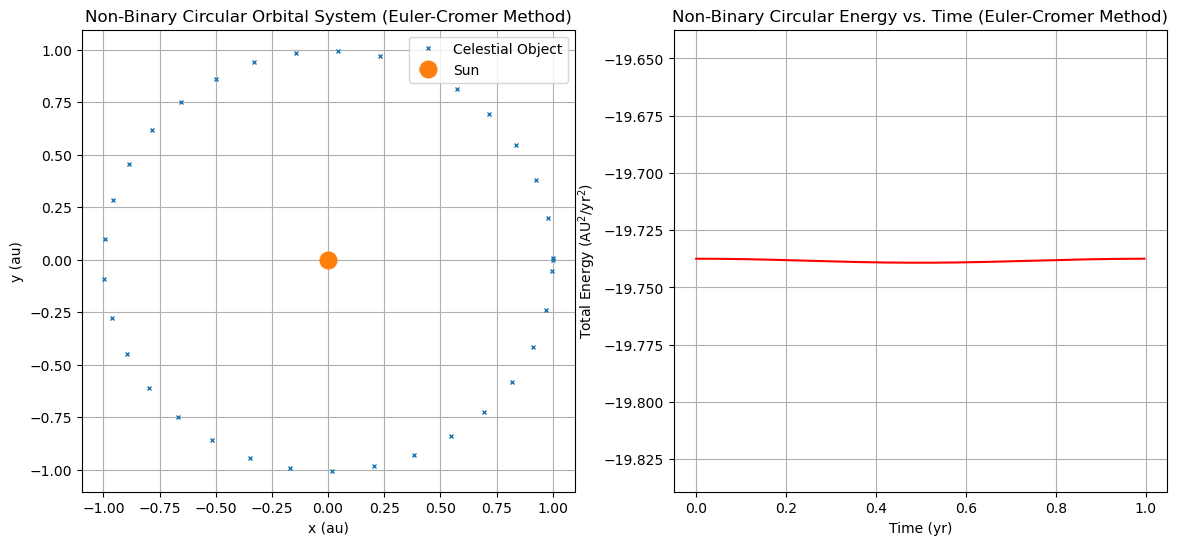
\includegraphics[width=1\linewidth]{Euler cromer/eulercromercircular.png}
  \centering
  \caption{\textit{Circular orbit of the object with $x = 1$ AU and $v_y = 2\pi$ AU/yr using the Euler-Cromer method with its energy-time graph.}} 
\end{figure}
The orbit graph clearly shows a circular orbit with a radius of 1 AU. However, the energy-time graph shows a small dip, showing that energy is not strongly conserved over a long period of time in this method
Figure 2 shows the circular orbit created using the RK2 method.
\begin{figure}[H] 
  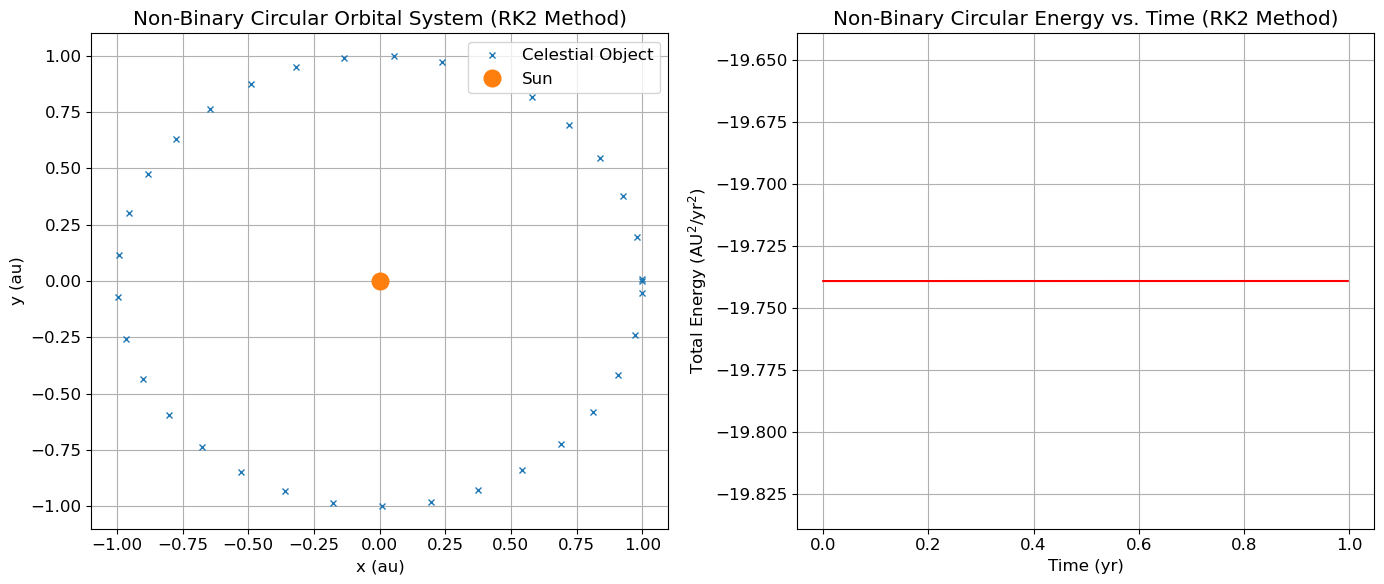
\includegraphics[width=1\linewidth]{RK2/rk2circular.png}
  \centering
  \caption{\textit{Circular orbit of the object with $x = 1$ AU and $v_y = 2\pi$ AU/yr using the RK2 method with its energy-time graph.}}
\end{figure}
The orbit graph once again shows a clear circle with the radius of 1 AU using the RK2 method with the energy-time graph showing a straight line, indicating that energy is conserved.

Figure 3 shows the circular orbit created using the leapfrog method.
\begin{figure}[H]
  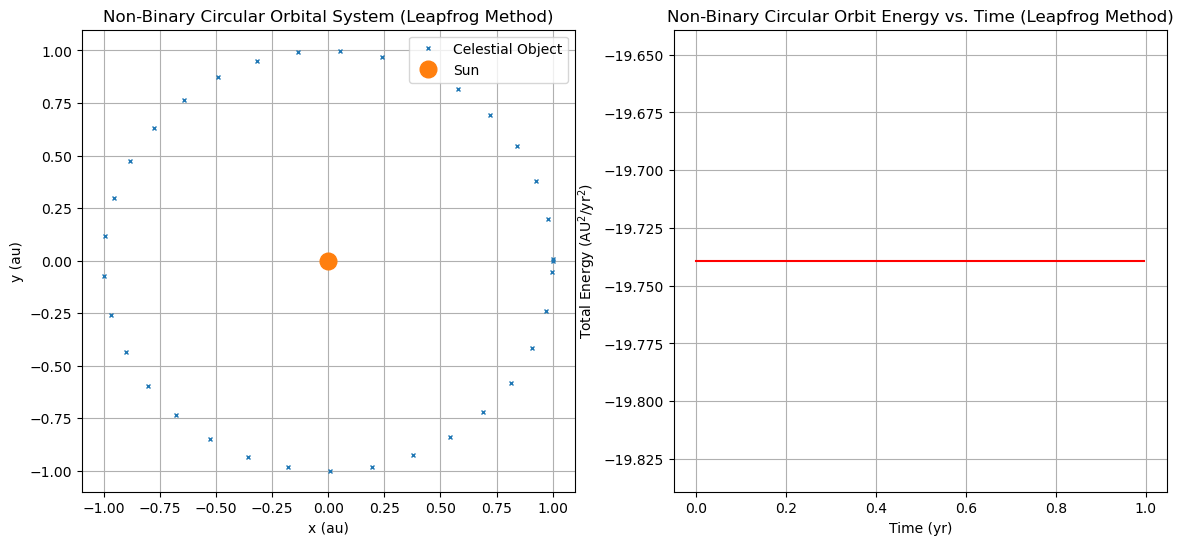
\includegraphics[width=1\linewidth]{Leapfrog/leapfrogcircular.png}
  \centering
  \caption{\textit{Circular orbit of the object with $x = 1$ AU and $v_y = 2\pi$ AU/yr using the leapfrog method with its energy-time graph.}}
\end{figure}
The orbit graph shapes to a cirle with a radius of 1 AU. With this method, the energy-time graph showed a straight line indicating the conservation of energy.

\subsubsection{Elliptical Orbits}
The methods were also used to create elliptical orbits of the object travelling around a non-binary system. The inital conditions for the orbital method
were $x=1$ AU and $v_y = \pi$ AU/yr.

Figure 4 shows the elliptical orbit of the object created using the Euler-Cromer method.
\begin{figure}[H]
  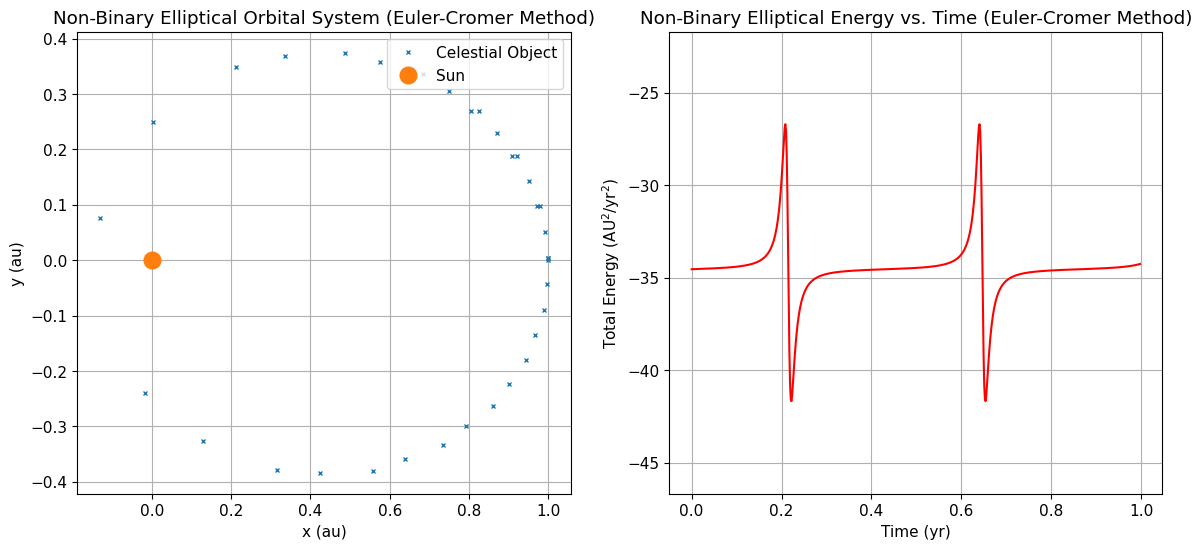
\includegraphics[width=1\linewidth]{Euler cromer/eulercromerelliptic.png}
  \centering
  \caption{\textit{Elliptical orbit of the object with $x = 1$ AU and $v_y = \pi$ AU/yr using the Euler-Cromer method and the energy-time graph.}} 
\end{figure}
The orbit graph shows an elliptical orbit but with a slight deviation after a certain time. This is also shown on the energy-time graph as the energy values drift away and then stabilise again, creating a tangential graph.

Figure 5 shows the elliptical orbit of the object created using the RK2 method.
\begin{figure}[H]
  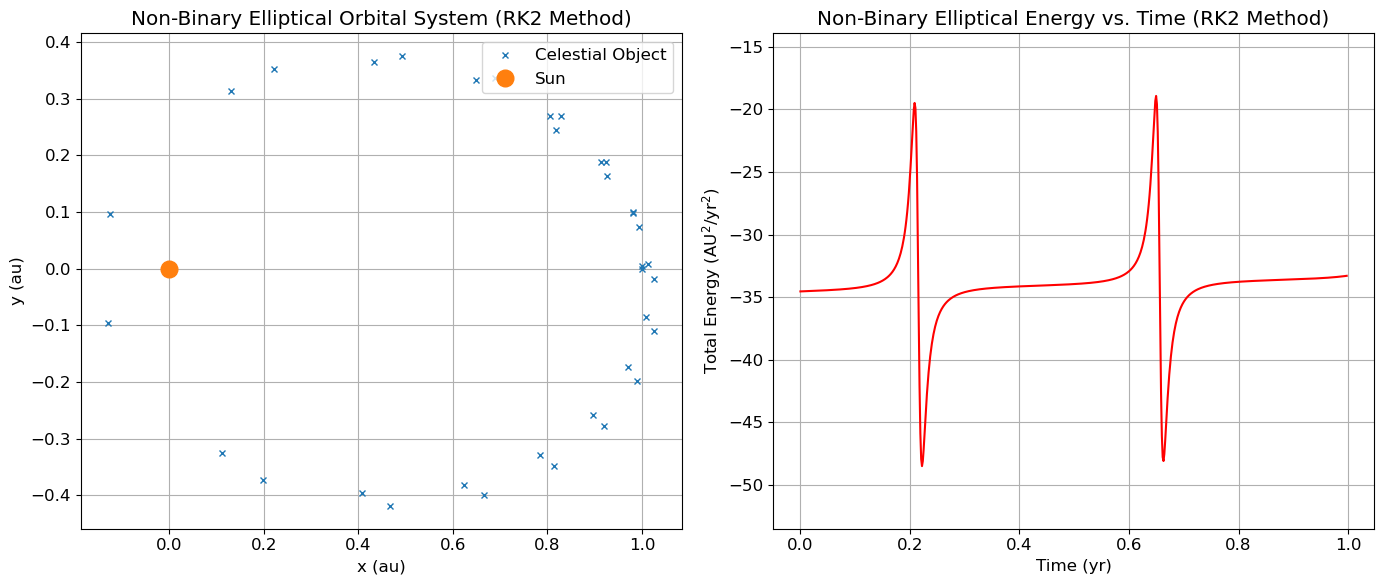
\includegraphics[width=1\linewidth]{RK2/rk2elliptic.png}
  \centering
  \caption{\textit{Elliptical orbit of the object with $x = 1$ AU and $v_y = \pi$ AU/yr using the RK2 method and the energy-time graph.}} 
\end{figure}


\begin{figure}[H]
  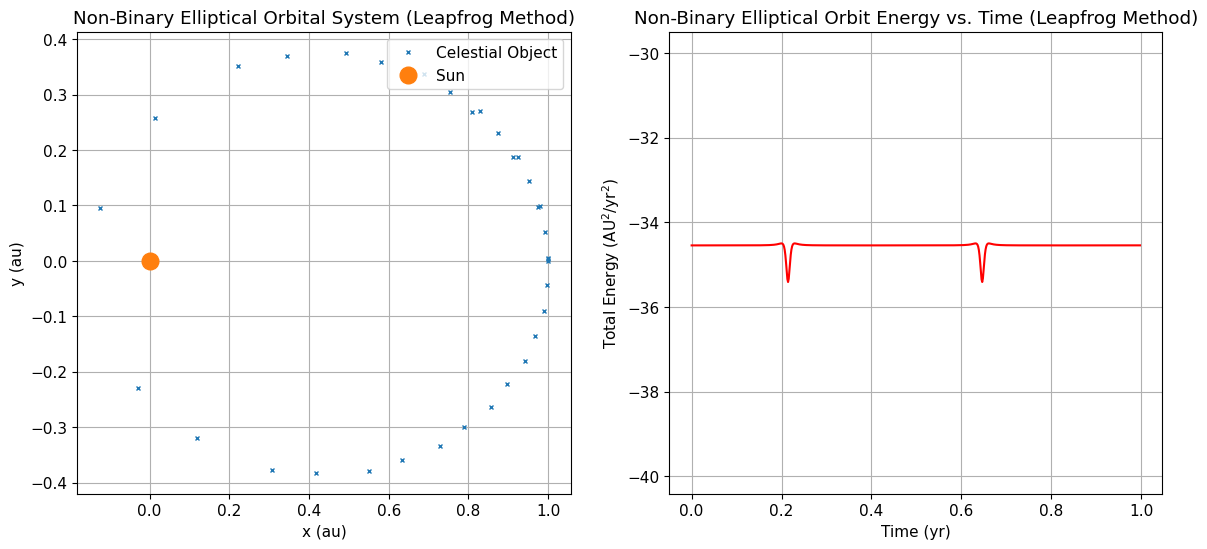
\includegraphics[width=1\linewidth]{Leapfrog/leapfrogelliptic.png}
  \centering
  \caption{\textit{The energy-time graph of an elliptical orbit with the initial conditions as in Figure 5 created using the RK2 method.}}
\end{figure}

\subsection{Effect of Time Step}
\subsubsection{Circular Orbits}
\begin{figure}[H]
  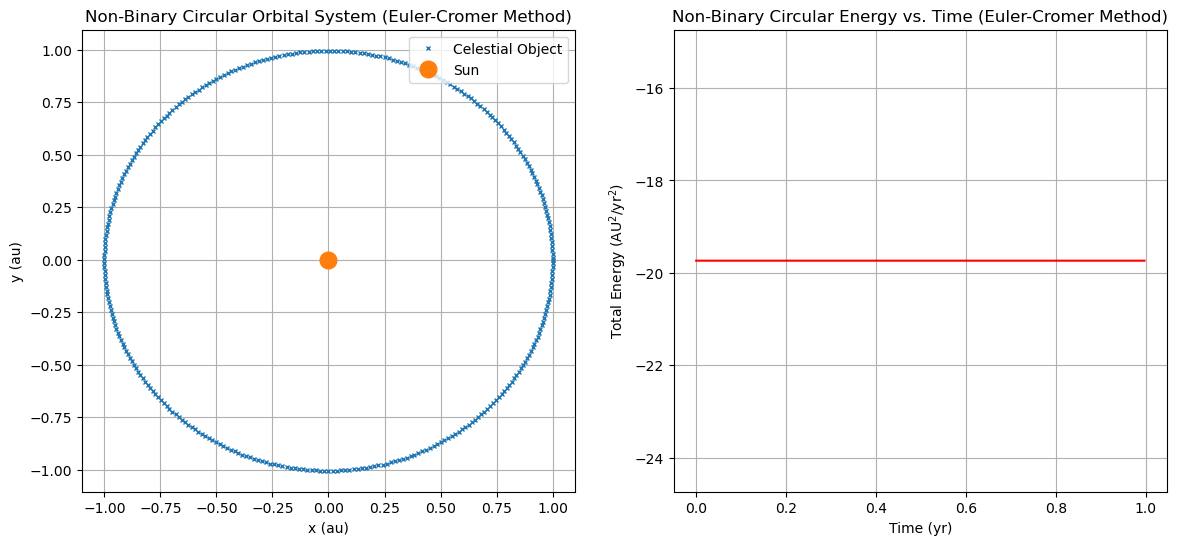
\includegraphics[width=0.7\linewidth]{Euler cromer/eulercromercircularincrease.png}
  \centering
  \caption{\textit{Circular orbit of the object with $x = 1$ AU and $v_y = 2\pi$ AU/yr using the Euler-Cromer method with decreased snaps with the energy-time graph.}} 
\end{figure}

\begin{figure}[H]
  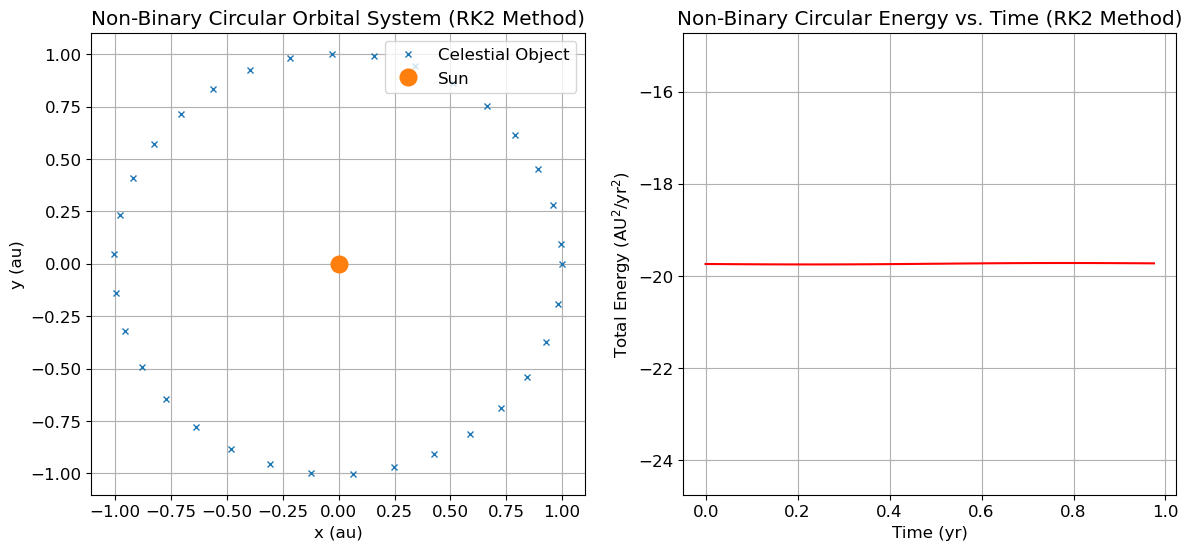
\includegraphics[width=0.7\linewidth]{RK2/rk2circularincrease.png}
  \centering
  \caption{\textit{Circular orbit of the object with $x = 1$ AU and $v_y = 2\pi$ AU/yr using the RK2 method with decreased snaps with the energy-time graph.}} 
\end{figure}

\begin{figure}[H]
  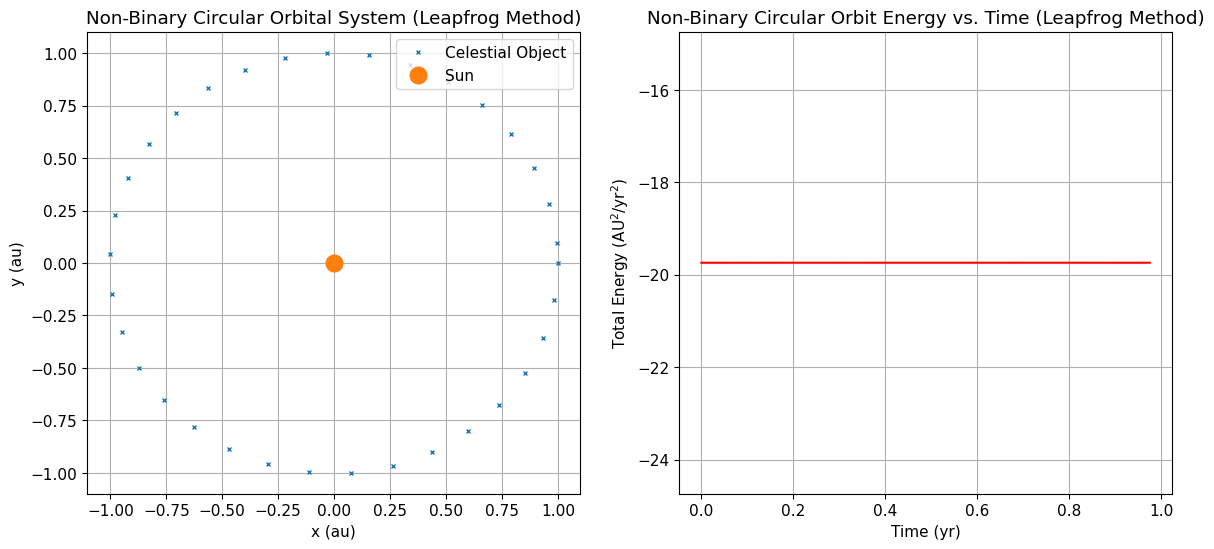
\includegraphics[width=0.7\linewidth]{Leapfrog/leapfrogcircularincrease.png}
  \centering
  \caption{\textit{Circular orbit of the object with $x = 1$ AU and $v_y = 2\pi$ AU/yr using the Leapfrog method with decreased snaps with the energy-time graph.}} 
\end{figure}

\subsubsection{Elliptical Orbits}
\begin{figure}[H]
  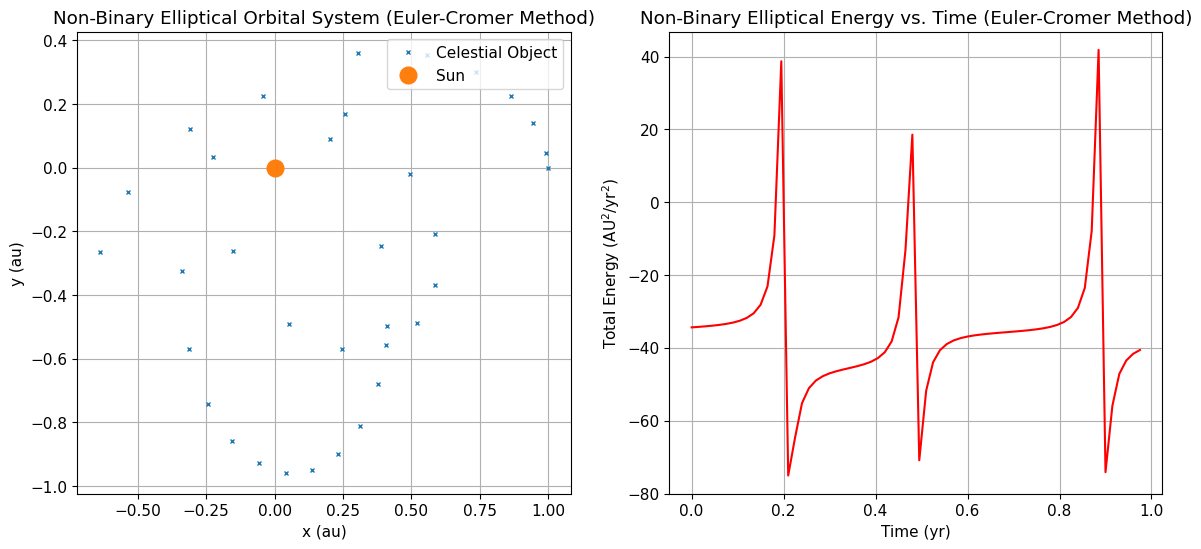
\includegraphics[width=0.7\linewidth]{Euler cromer/eulercromerellipticincrease.png}
  \centering
  \caption{\textit{Elliptical orbit of the object with $x = 1$ AU and $v_y = 2\pi$ AU/yr using the Euler-Cromer method with decreased snaps with the energy-time graph.}} 
\end{figure}

\begin{figure}[H]
  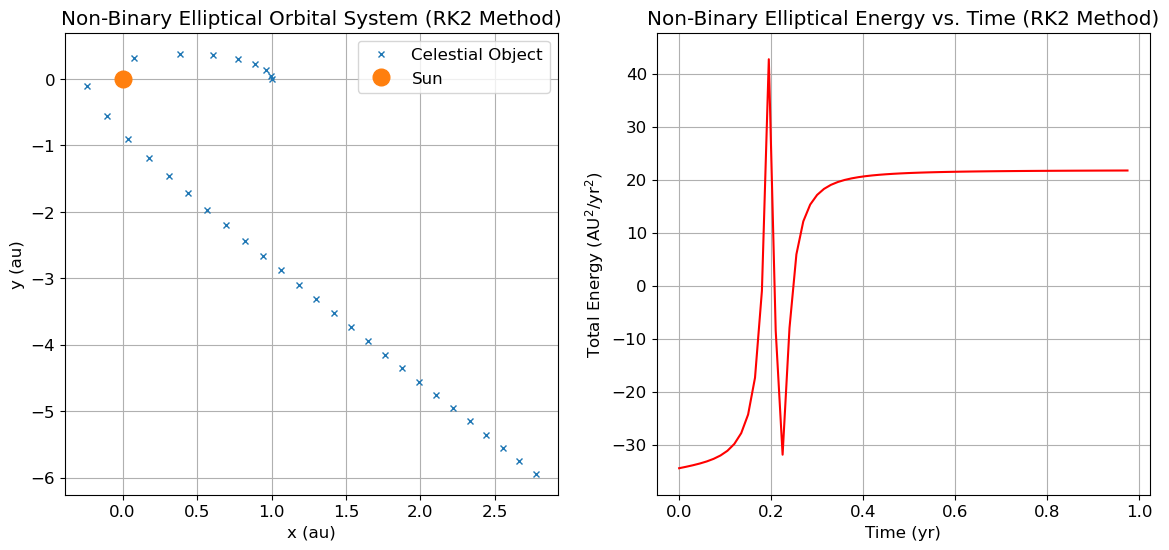
\includegraphics[width=0.7\linewidth]{RK2/rk2ellipticincrease.png}
  \centering
  \caption{\textit{Elliptical orbit of the object with $x = 1$ AU and $v_y = 2\pi$ AU/yr using the RK2 method with decreased snaps with the energy-time graph.}} 
\end{figure}

\begin{figure}[H]
  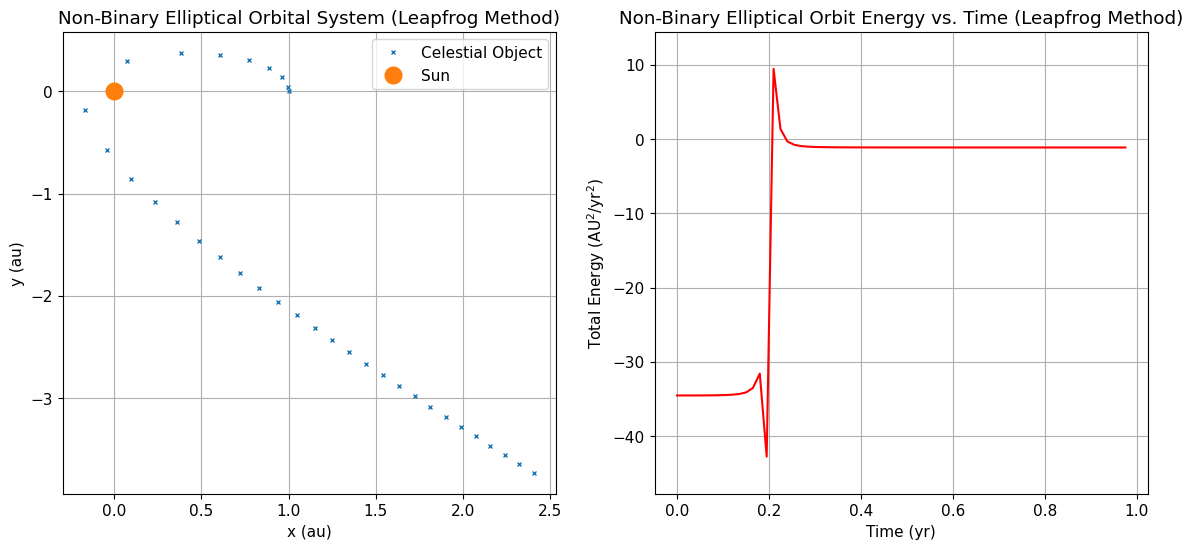
\includegraphics[width=0.7\linewidth]{Leapfrog/leapfrogellipticincrease.png}
  \centering
  \caption{\textit{Elliptical orbit of the object with $x = 1$ AU and $v_y = 2\pi$ AU/yr using the Leapfrog method with decreased snaps with the energy-time graph.}} 
\end{figure}

\subsection{Numerical intergration in a Binary System}
\subsubsection{Circular Orbits}

\begin{figure}[H]
  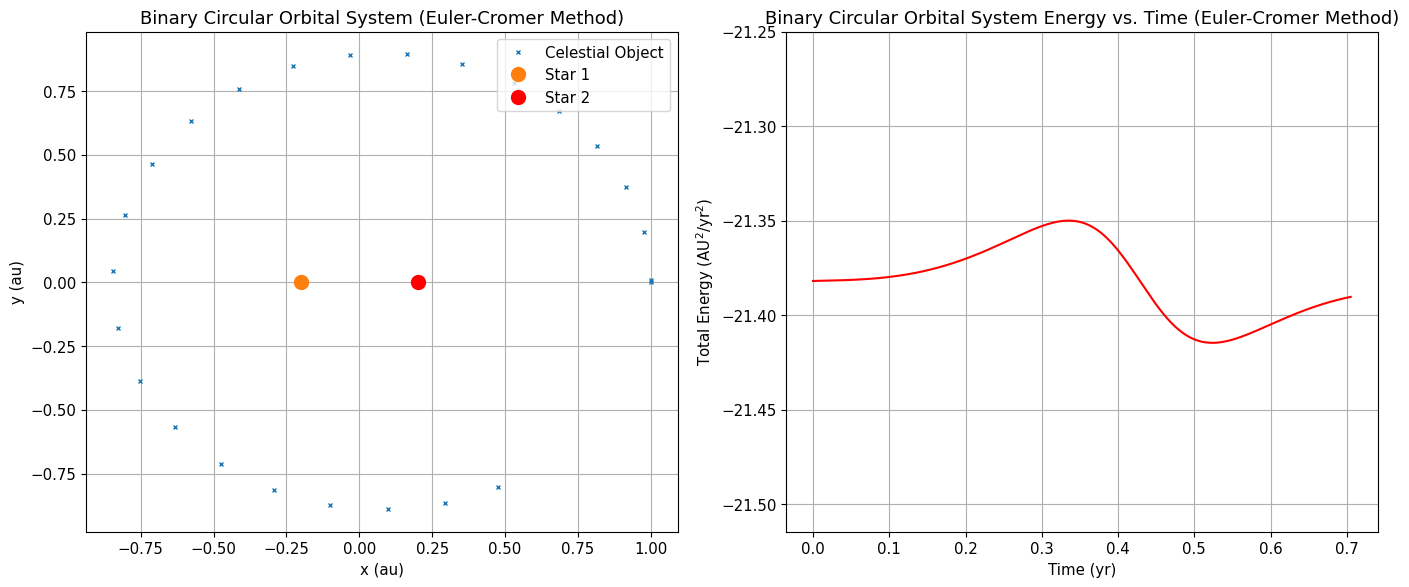
\includegraphics[width=0.7\linewidth]{binaryeulercircular.png}
  \centering
  \caption{\textit{Binary circular orbit of the object with $x = 1$ AU and $v_y = 2\pi$ AU/yr using the Euler-Cromer method with decreased snaps with the energy-time graph.}} 
\end{figure}

\begin{figure}[H]
  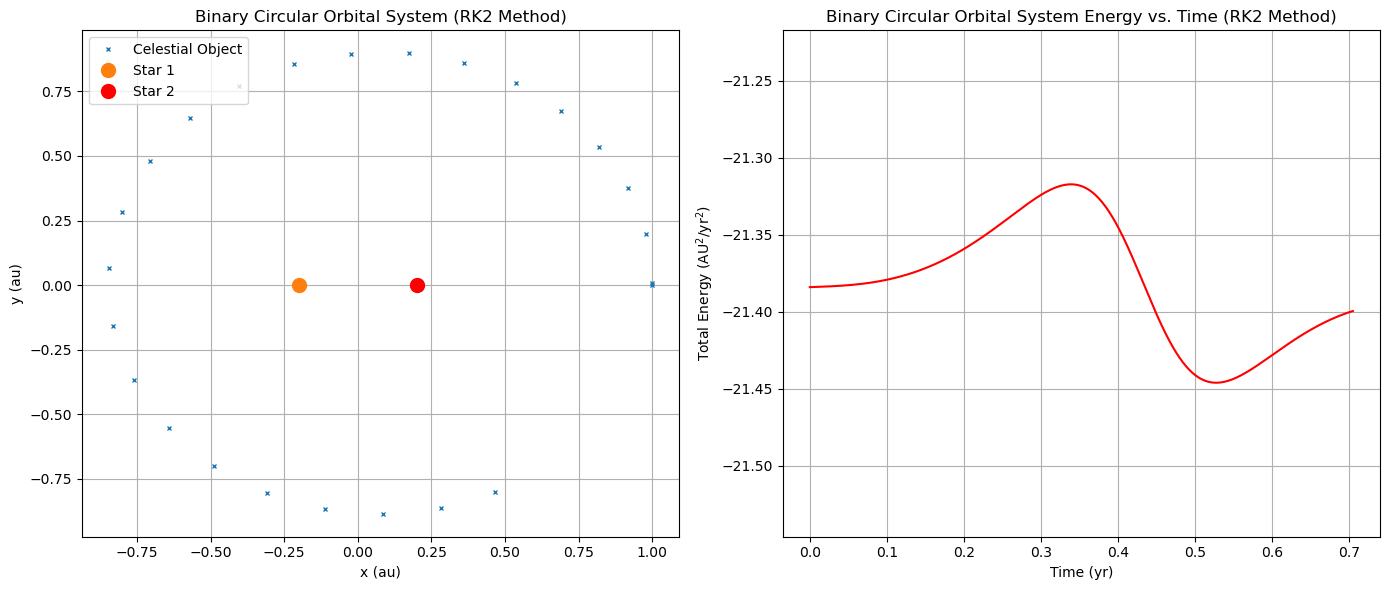
\includegraphics[width=0.7\linewidth]{binaryrk2circular.png}
  \centering
  \caption{\textit{Binary circular orbit of the object with $x = 1$ AU and $v_y = 2\pi$ AU/yr using the RK2 method with decreased snaps with the energy-time graph.}} 
\end{figure}

\begin{figure}[H]
  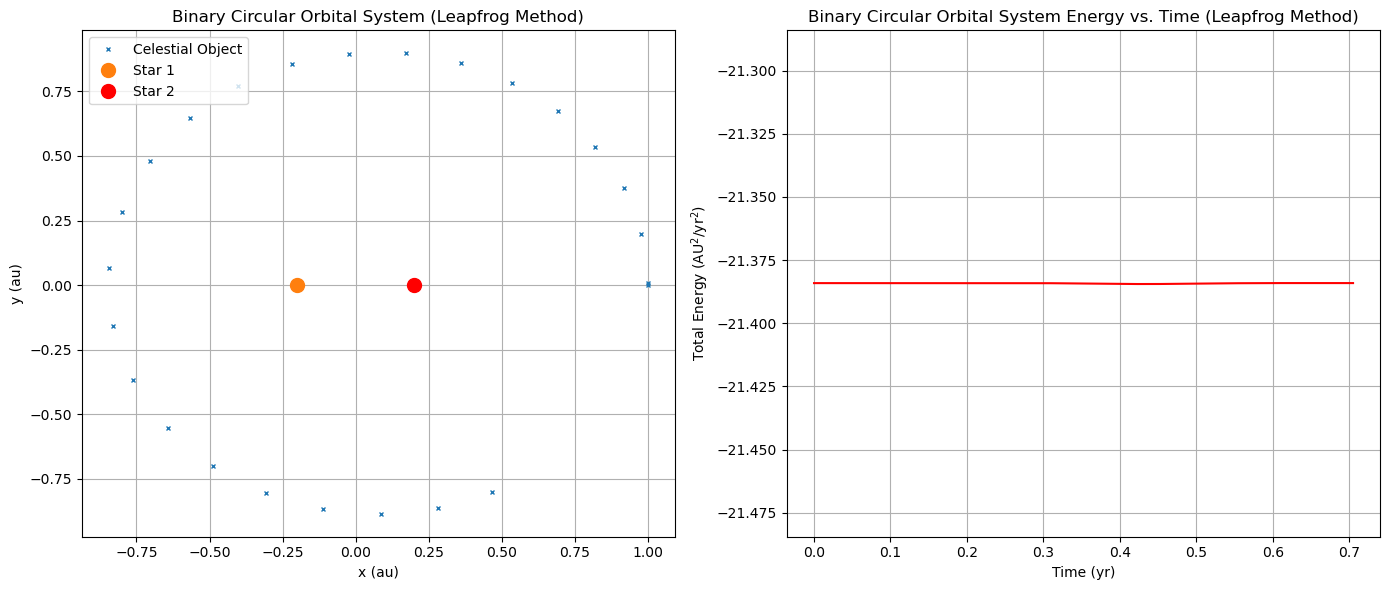
\includegraphics[width=0.7\linewidth]{binaryleapfrogcircular.png}
  \centering
  \caption{\textit{Binary circular orbit of the object with $x = 1$ AU and $v_y = 2\pi$ AU/yr using the leapfrog method with decreased snaps with the energy-time graph.}} 
\end{figure}

\subsubsection{Elliptical Orbits}
\begin{figure}[H]
  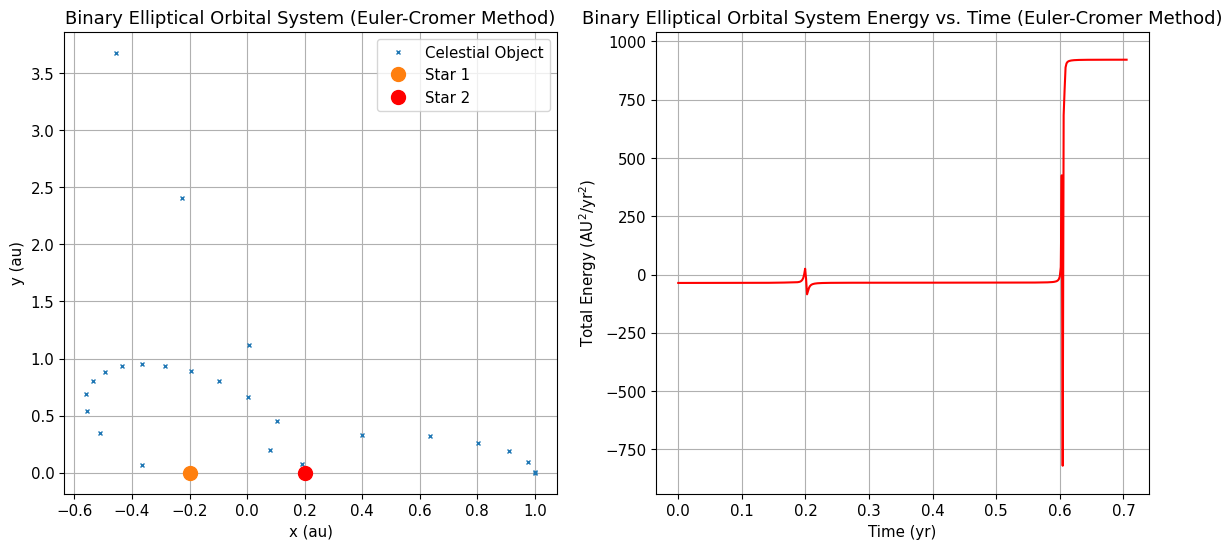
\includegraphics[width=0.7\linewidth]{binaryeulerelliptic.png}
  \centering
  \caption{\textit{Circular orbit of the object with $x = 1$ AU and $v_y = 2\pi$ AU/yr using the Euler-Cromer method with decreased snaps with the energy-time graph.}} 
\end{figure}

\begin{figure}[H]
  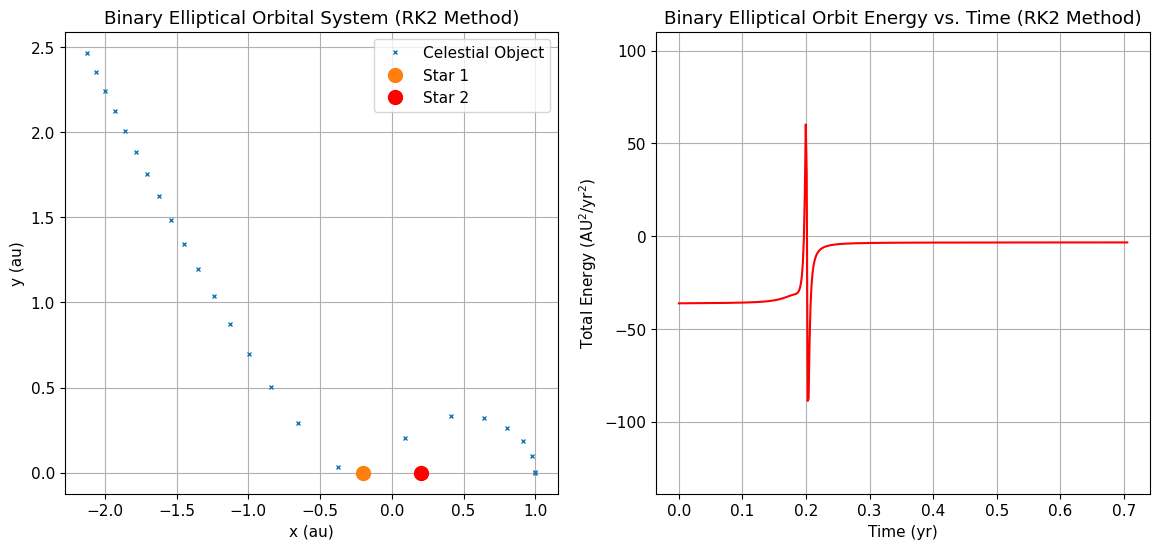
\includegraphics[width=0.7\linewidth]{binaryrk2elliptic.png}
  \centering
  \caption{\textit{Circular orbit of the object with $x = 1$ AU and $v_y = 2\pi$ AU/yr using the Euler-Cromer method with decreased snaps with the energy-time graph.}} 
\end{figure}

\begin{figure}[H]
  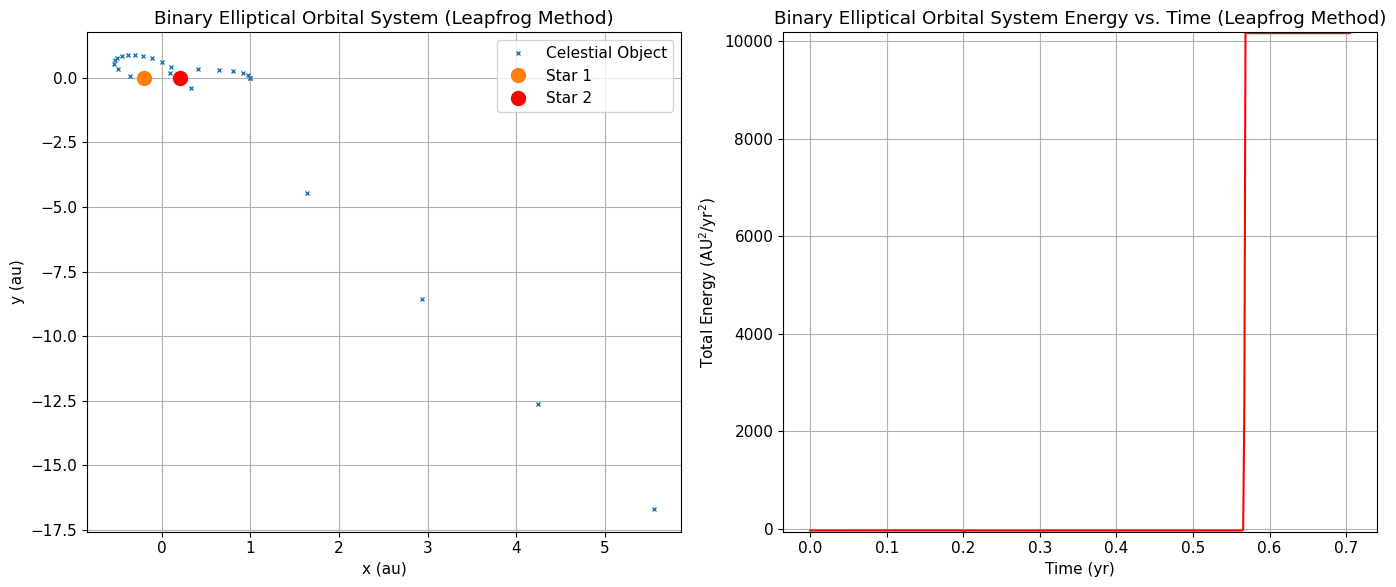
\includegraphics[width=0.7\linewidth]{binaryleapfrogelliptic.png}
  \centering
  \caption{\textit{Circular orbit of the object with $x = 1$ AU and $v_y = 2\pi$ AU/yr using the Euler-Cromer method with decreased snaps with the energy-time graph.}} 
\end{figure}

\section{Discussion}
From the three graphs presented under the circular orbits, it can be seen that all intergration methods works well, preserving the law of conservation of energy and angular momentum.
This was expected as circular orbit means that the energies are constant, resulting in a constant sum. The Euler-Cromer sees a small dip which shows that energy is not properly conserved at long periods of time.


\section{Conclusion}
A

\newpage
\section{References}  

[1] NASA. "Chapter 7 Fundamentals of Orbital Mechanics." NASA. Accessed: 19 Sept. 2025. [Online]. Available: \url{https://spsweb.fltops.jpl.nasa.gov/portaldataops/mpg/MPG_Docs/MPG%20Book/Release/Chapter7-OrbitalMechanics.pdf}.

[2] \url{https://phys.libretexts.org/Bookshelves/Conceptual_Physics/Introduction_to_Physics_(Park)/02%3A_Mechanics_I_-_Motion_and_Forces/02%3A_Dynamics/2.09%3A_Newtons_Universal_Law_of_Gravitation}

[3] \url{https://www.sciencedirect.com/science/article/pii/B9780124158450000037}

[4] Exploring the system lab

[5] \url{https://orbital-mechanics.space/constants-of-orbital-motion/energy-is-conserved-in-orbital-motion.html}

[6] \url{chrome-extension://efaidnbmnnnibpcajpcglclefindmkaj/https://homepages.dias.ie/ydri/TP3-en.pdf}

[7] \url{chrome-extension://efaidnbmnnnibpcajpcglclefindmkaj/https://liceocuneo.it/oddenino/wp-content/uploads/sites/2/Alan-Cromer-Stable-solutions-using-the-Euler-Approximation-American-Journal-of-Physics-49-455-1981.pdf}

[8] \url{https://www.sciencedirect.com/science/article/pii/B9780128097304000276}

[9] \url{https://www.sciencedirect.com/science/article/pii/B9780128097304000276}

[10] \url{chrome-extension://efaidnbmnnnibpcajpcglclefindmkaj/https://www.colorado.edu/amath/sites/default/files/attached-files/sttime.pdf}

\newpage
\section{Appendix}

\subsection{Coding}
\subsubsection{The Euler-Cromer Method for a Non-Binary System}
\lstinputlisting[language=Python]{Euler cromer/euleronestar.py}

\subsubsection{The 2nd Order Runge-Kutta Method for a Non-Binary System}
\lstinputlisting[language=Python]{RK2/2rkonestar.py}

\subsubsection{The Leapfrog Method for a Non-Binary System}
\lstinputlisting[language=Python]{Leapfrog/leapfrogonestar.py}

\end{document}
